
\section{Paweł Lorenc}
\label{sec:plorenc}



\textbf{\textit{Prawo Ohma}}

\centering \textbf{dla obwodu prądu stałego mamy}:
\begin{equation}
    U = I \cdot R
\end{equation}
gdzie:
\begin{itemize}
    \item \(U\) – napięcie elektryczne (wolt),
    \item \(I\) – natężenie prądu (amper),
    \item \(R\) – opór elektryczny (om).
\end{itemize}

\subsection{Obraz}
Poniżej przedstawiono przykład obwodu prądu stałego (zobacz Rysunek~\ref{fig:obwod}). 

\begin{figure}[htp]
    \centering
    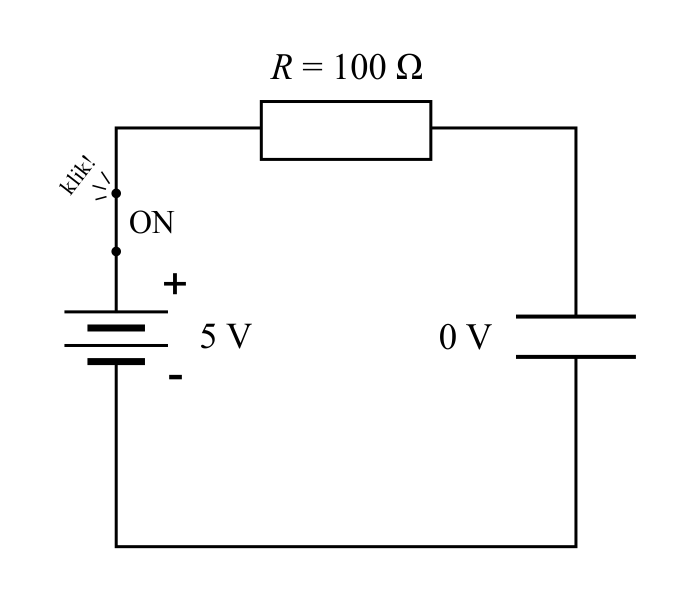
\includegraphics[width=0.5\linewidth]{pictures/zamkniecie-obwodu-kondensatora.png}
    \caption{Obwód prądu stałego}
    \label{fig:obwod}
\end{figure}
\
Obwód przedstawiony na rysunku pokazuje przepływ prądu przez rezystor w warunkach stałego napięcia.

\newpage

\subsection{Tabela}
Tabela~\ref{tab:prad_napiecie} prezentuje przykładowe wartości prądu i napięcia w obwodzie.

\begin{table}[h]
    \centering
    \caption{Przykładowe wartości prądu i napięcia}
    \begin{tabular}{|c|c|}
        \hline
        Natężenie prądu (A) & Napięcie (V) \\
        \hline
        0.5 & 5 \\
        1.0 & 10 \\
        1.5 & 15 \\
        2.0 & 20 \\
        \hline
    \end{tabular}
    \label{tab:prad_napiecie}
\end{table}
\label{tab:tabelkaPL}


\subsection{Lista nienumerowana}
W odniesieniu do Tabeli~\ref{tab:prad_napiecie} przykładowe wartości można interpretować w następujący sposób:
\begin{itemize}
    \item 0.5 A - wartość prądu przy napięciu 5 V,
    \item 1.0 A - wartość prądu przy napięciu 10 V,
    \item 1.5 A - wartość prądu przy napięciu 15 V,
    \item 2.0 A - wartość prądu przy napięciu 20 V.
\end{itemize}
\~\

\
\section{Informacje o Prądzie Elektrycznym}

Prąd elektryczny to przepływ ładunków elektrycznych przez przewodnik, który zachodzi pod wpływem przyłożonego napięcia. W układach prądu stałego, kierunek przepływu ładunków jest stały, co odróżnia go od prądu zmiennego, gdzie kierunek i natężenie prądu zmieniają się cyklicznie. Natężenie prądu oznacza się symbolem \( I \) i mierzy w jednostkach ampera (A), co wskazuje ilość ładunku przepływającego przez przekrój przewodnika w jednostce czasu.

Wartość prądu zależy od oporu przewodnika i napięcia zgodnie z prawem Ohma, które określa, że natężenie prądu jest równe stosunkowi napięcia \( U \) do oporu \( R \): \( I = \frac{U}{R} \). Prąd elektryczny odgrywa kluczową rolę w działaniu urządzeń elektronicznych, a jego kontrolowanie pozwala na bezpieczne i efektywne korzystanie z energii elektrycznej.


\begin{center}
    
\end{center}

